\section{Airport Locations}
Map showing the locations of all airports in the Chicago area, with a 100-mile radius circle around Chicago.
\begin{figure}[htbp]
\centering
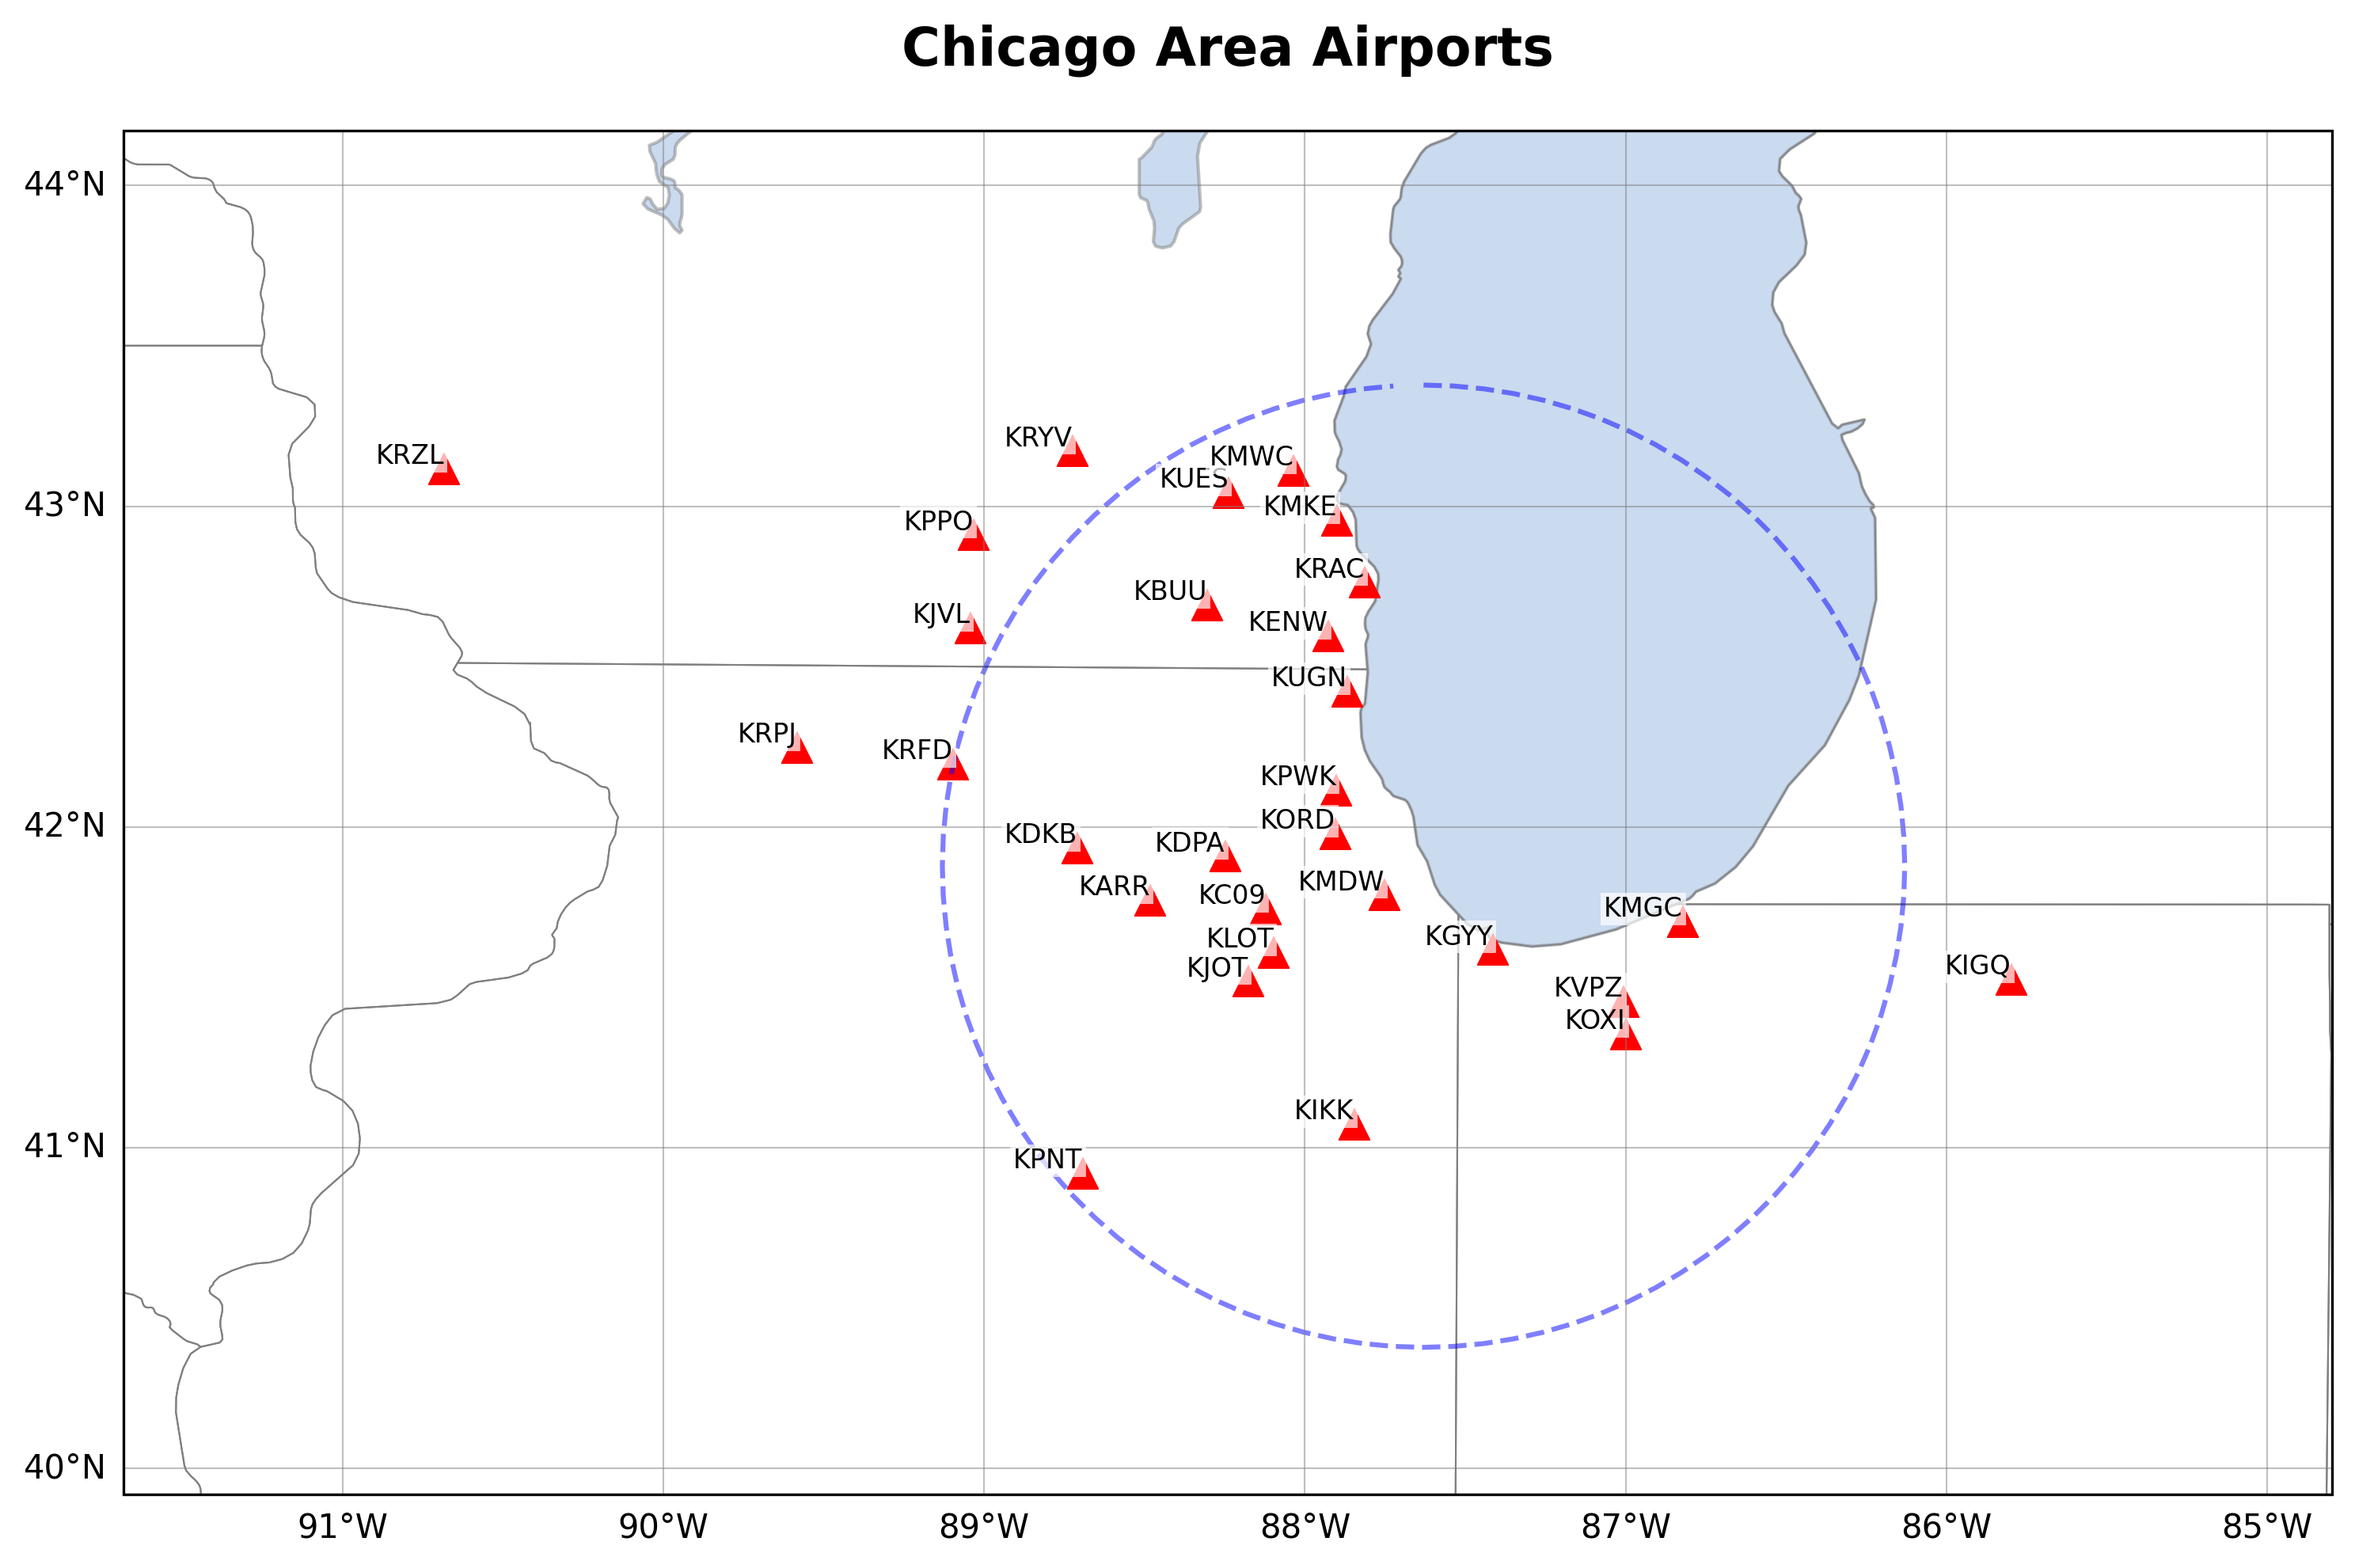
\includegraphics[width=0.7	extwidth]{airport_map.png}
\caption{Chicago Area Airports}
\label{fig:airport_map}
\end{figure}
\section{Airport Table}
\begin{tabular}{lllrr}
\toprule
 & Code & Name & Latitude & Longitude \\
\midrule
0 & KORD & Chicago O'Hare & 41.98 & -87.90 \\
1 & KMDW & Chicago Midway & 41.79 & -87.75 \\
2 & KMKE & Milwaukee & 42.95 & -87.90 \\
3 & KPWK & Chicago Executive & 42.11 & -87.90 \\
4 & KDPA & DuPage & 41.91 & -88.25 \\
5 & KGYY & Gary & 41.62 & -87.41 \\
6 & KRFD & Chicago Rockford & 42.20 & -89.10 \\
7 & KARR & Aurora Municipal & 41.77 & -88.48 \\
8 & KUGN & Waukegan & 42.42 & -87.87 \\
9 & KVPZ & Porter County & 41.45 & -87.01 \\
10 & KJOT & Joliet Regional & 41.52 & -88.18 \\
11 & KIKK & Greater Kankakee & 41.07 & -87.85 \\
12 & KENW & Kenosha Regional & 42.60 & -87.93 \\
13 & KRAC & Racine & 42.76 & -87.81 \\
14 & KBUU & Burlington Municipal & 42.69 & -88.30 \\
15 & KJVL & Southern Wisconsin Regional & 42.62 & -89.04 \\
16 & KDKB & DeKalb Taylor Municipal & 41.93 & -88.71 \\
17 & KRYV & Watertown Municipal & 43.17 & -88.72 \\
18 & KRZL & Reedsburg Municipal & 43.12 & -90.68 \\
19 & KUES & Waukesha County & 43.04 & -88.24 \\
20 & KC09 & Plainfield & 41.74 & -88.12 \\
21 & KIGQ & Boone County & 41.52 & -85.80 \\
22 & KLOT & Lewis University & 41.61 & -88.10 \\
23 & KMGC & Michigan City Municipal & 41.70 & -86.82 \\
24 & KMWC & Milwaukee-Timmerman & 43.11 & -88.03 \\
25 & KOXI & Starke County & 41.35 & -87.00 \\
26 & KPNT & Pontiac Municipal & 40.92 & -88.69 \\
27 & KPPO & Poplar Grove & 42.91 & -89.03 \\
28 & KRPJ & Rochelle Municipal & 42.25 & -89.58 \\
\bottomrule
\end{tabular}

